\section{Development Method}
\label{sec:DevelopmentMethods}
In this section we will describe a few different Software delvelopmentmoethods that we considered using.

\subsection{Waterfall}
The waterfall method, first published by Dr. Winston W. Royse in 1970, has derived its name directly from the concept of the method. If following this method in it's traditional form, development will go through several completely separated steps, from which it is never possible to go back (see \ref{fig:WaterfallPic}). These steps will not necessarily be done by the same development teams which means that everything has to be documented thoroughly before starting the next step.\\
 \\
Royce originally ment for this method to be developed into a fully iterative model, however, most software developers adapted to non-iterative form.
\cite{waterfallroyce}

\begin{figure}[H]
	\centering
		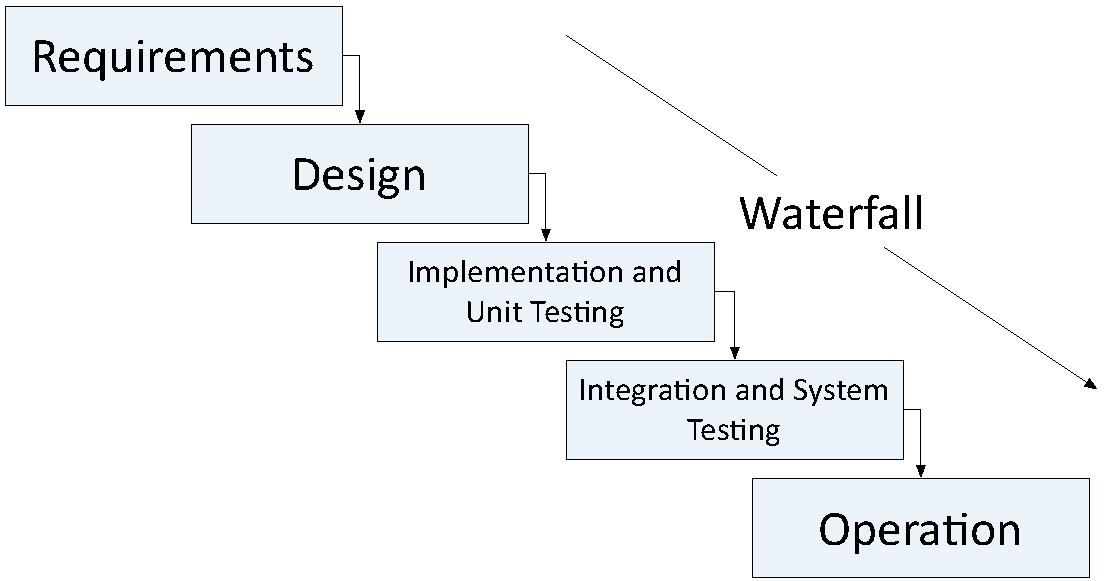
\includegraphics[width=0.90\textwidth]{input/implementation/development/waterfall.pdf}
	\morscaption{This illustrates a traditional waterfall in which the "water" can only proceed downwards untill reaching the end (process completetion)}
	\label{fig:WaterfallPic}
\end{figure}

\subsection{Agile Methods}